%!TEX root = index.tex
\chapter{Analises}
\label{cha:analises}

\section{Samsung}

A partir de conversas com Luís Guilherme Selber, responsável pela operação do Laboratório Ocean, obtivemos a seguinte análise:

\begin{figure}[H]
\caption{Análise do Ocean - Samsung}
\centerline{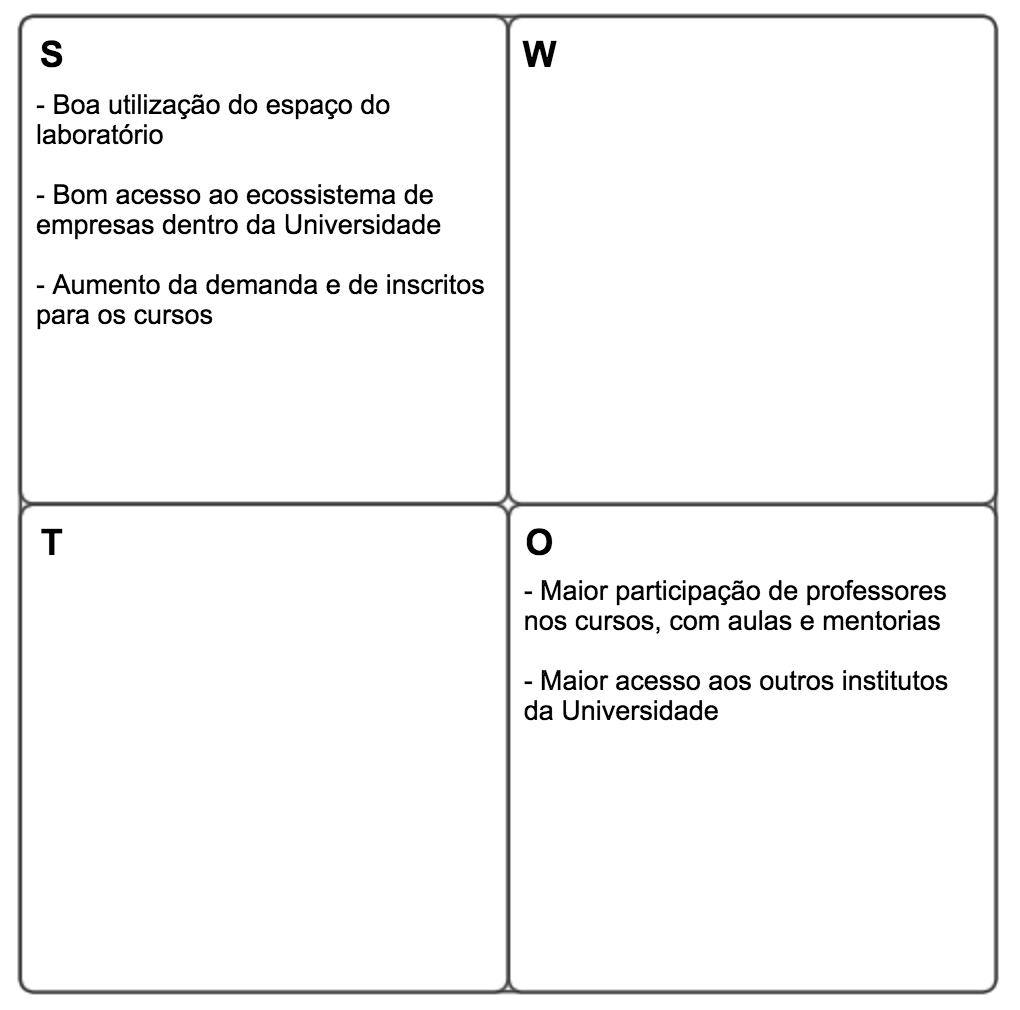
\includegraphics[scale=0.75]{img/samsungswot}}
\label{fig:swotsamsung}
\caption* {Fonte: Elaborado pelo próprio autor}
\end{figure}

A ausência de fraquezas e ameaças se dá - segundo o entrevistado - pelo fato de o projeto estar em uma fase inicial. Não há formalidades estabelecidas como reuniões periódicas, quando é necessário conversar sobre algo é fácil encontrar um professor no corredor ou em sua sala, portanto as interações se limitam às necessidades de um ou outro, sem conflitos até o momento. A própria gestão de uso do Laboratório para as atividades de cada instituição não gera conflitos pois as necessidades de uso do laboratório por cada parte já foram claramente estabelecidas nas reuniões iniciais de fechamento do projeto.

Em relação aos pontos fortes, destaca-se o fato de o laboratório sofrer uma mudança muito positiva devido à mudança de localidade para dentro da universidade. A presença do laboratório dentro do PRO mudou completamente a utilização do laboratório, que agora é ocupado das 08 da manhã até as 22 da noite de segunda a sexta, fato que não acontecia na Faria Lima. Quando na Av. Brigadeiro Faria Lima, a Samsung exercia um papel ativo de sediar eventos próprios ou externos com o intuito de divulgar e preencher o espaço do laboratório. Tudo isso porque mais pessoas utilizando o espaço ajuda a divulgar mais o programa e os cursos oferecidos pelo laboratório. Não obstante, além dos próprios cursos dados pelo laboratório, ainda existe um custo com equipamentos e internet que não deveria existir em vão.

2. A USP é um ecossistema de parcerias com diversas empresas. O fato de estar dentro da Universidade por si só já coloca a Samsung em contato mais próximo com outras empresas, tendo provido reuniões com outras grandes empresas do mercado nacional.

3. Aumento da Demanda e de inscrições nos cursos intensivos, graças a participação de alunos e ex-alunos da própria universidade. 

- Cogestão Poli - Ocean

Situação atual: Ainda está baseado em reuniões pontuais e conversas de corredor, ainda em fase inicial, sem problemas da parte da samsung.
Futuro: Ter reuniões periódicas baseadas para definir melhor a utilização do espaço, projetos conjuntos...

Sobre a questão de utilização do espaço, a Samsung acredita que não haverá problema em relação a utilização do espaço, pois foi previamente alinhado as necessidades do uso do espaço pela Samsung e pela Universidade, sendo esse um ponto crítico para a parceria ter se estabelecido. Portas retrateis podem dividir o laboratório permitindo até 2 cursos em paralelo. 

\section{PRO}

\begin{figure}[H]
\caption{Análise do Ocean - PRO}
\centerline{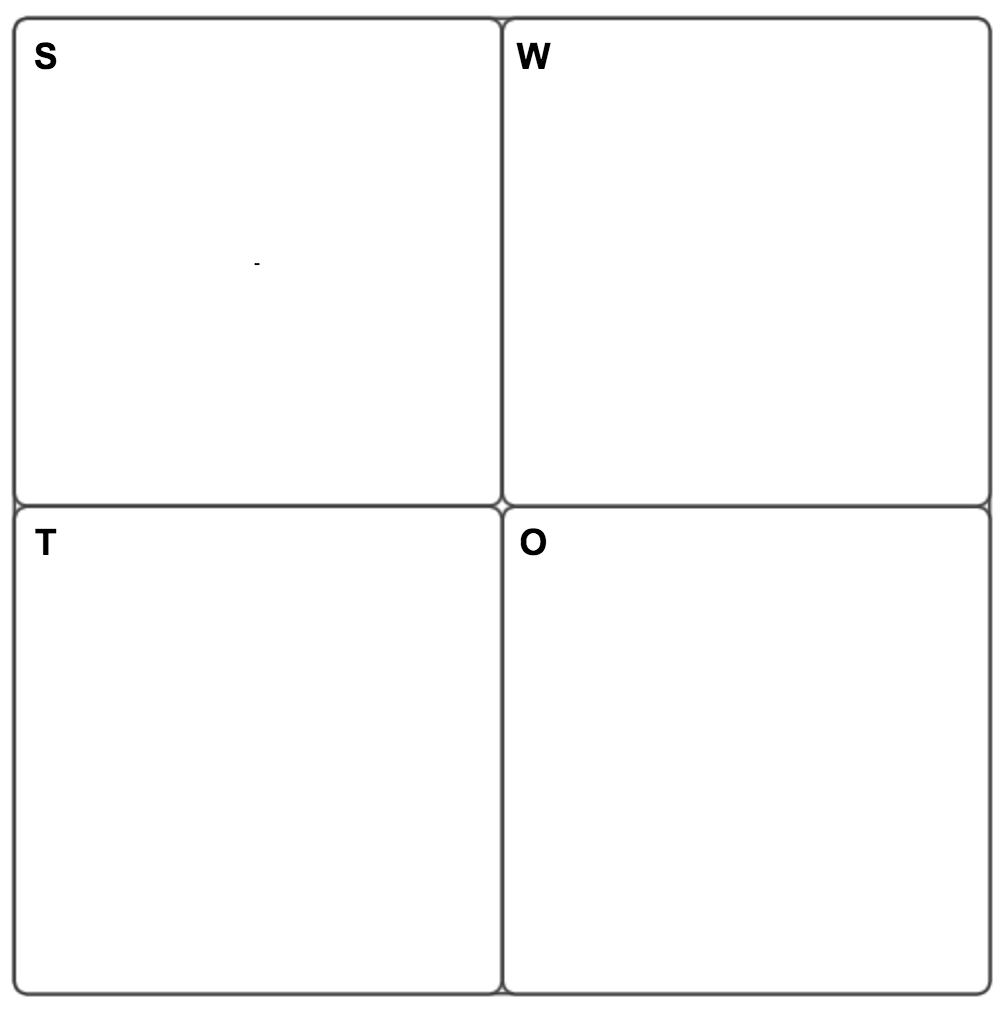
\includegraphics[scale=0.75]{img/generalswot}}
\label{fig:swotpro}
\caption* {Fonte: Elaborado pelo próprio autor}
\end{figure}

\section{NEU}

\begin{figure}[H]
\caption{Análise do Ocean - NEU}
\centerline{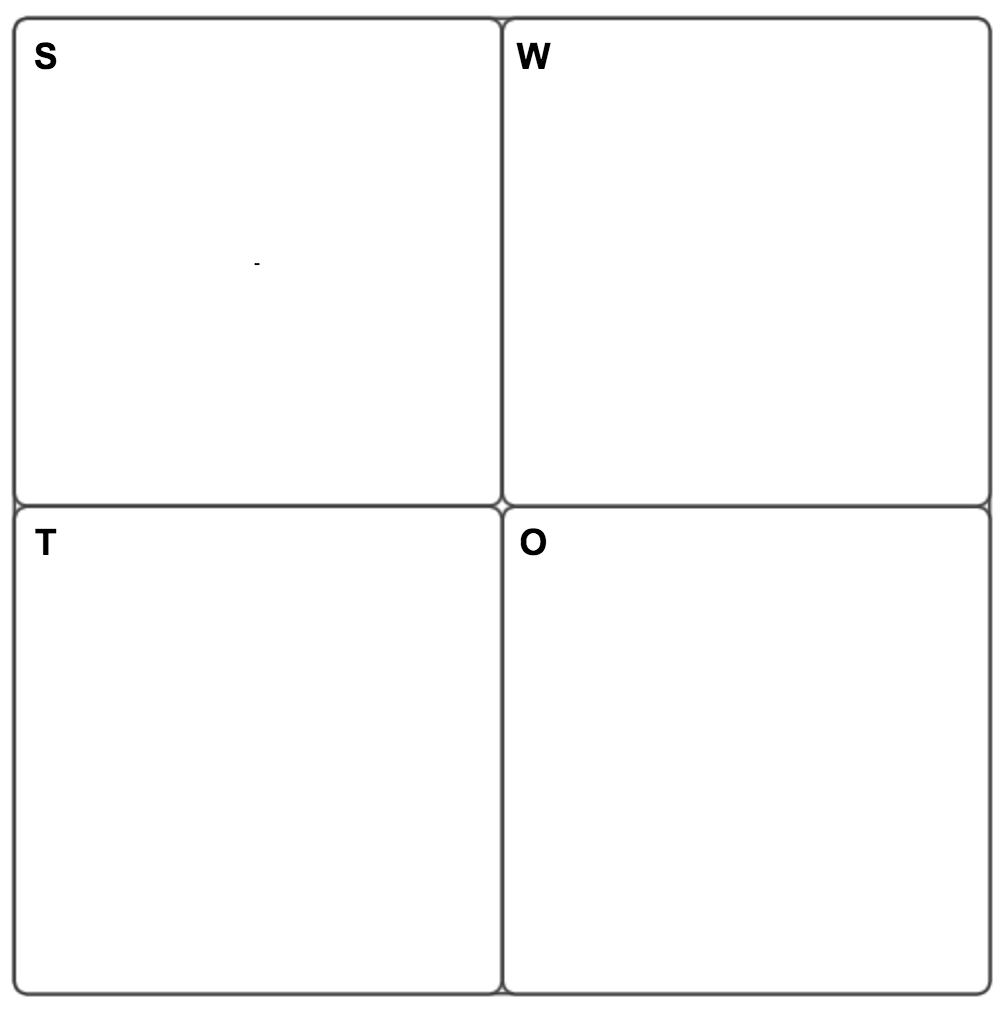
\includegraphics[scale=0.75]{img/generalswot}}
\label{fig:swotneu}
\caption* {Fonte: Elaborado pelo próprio autor}
\end{figure}

\section{Alunos}

\begin{figure}[H]
\caption{Análise do Ocean - Alunos}
\centerline{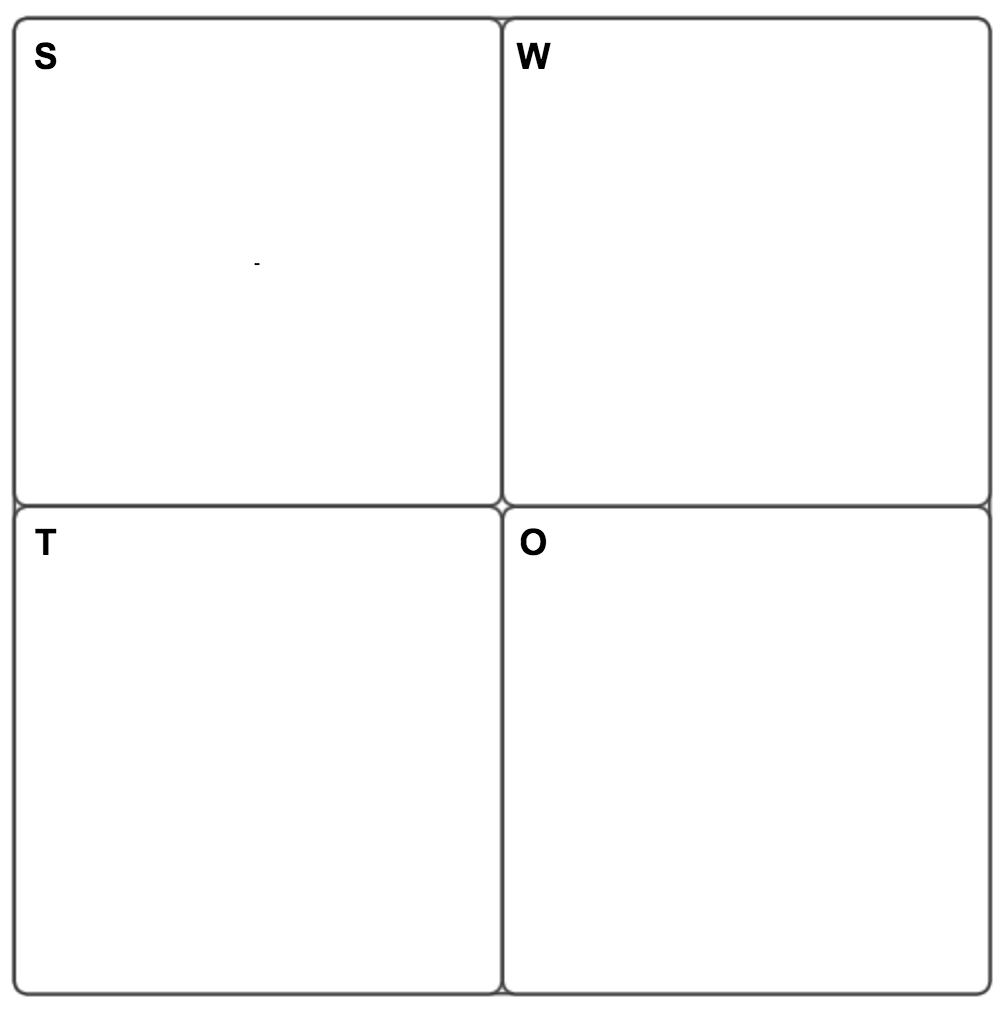
\includegraphics[scale=0.75]{img/generalswot}}
\label{fig:swotalunos}
\caption* {Fonte: Elaborado pelo próprio autor}
\end{figure}

\section{Usuários Externos}

\begin{figure}[h]
\caption{Análise do Ocean - Usuários Externos}
\centerline{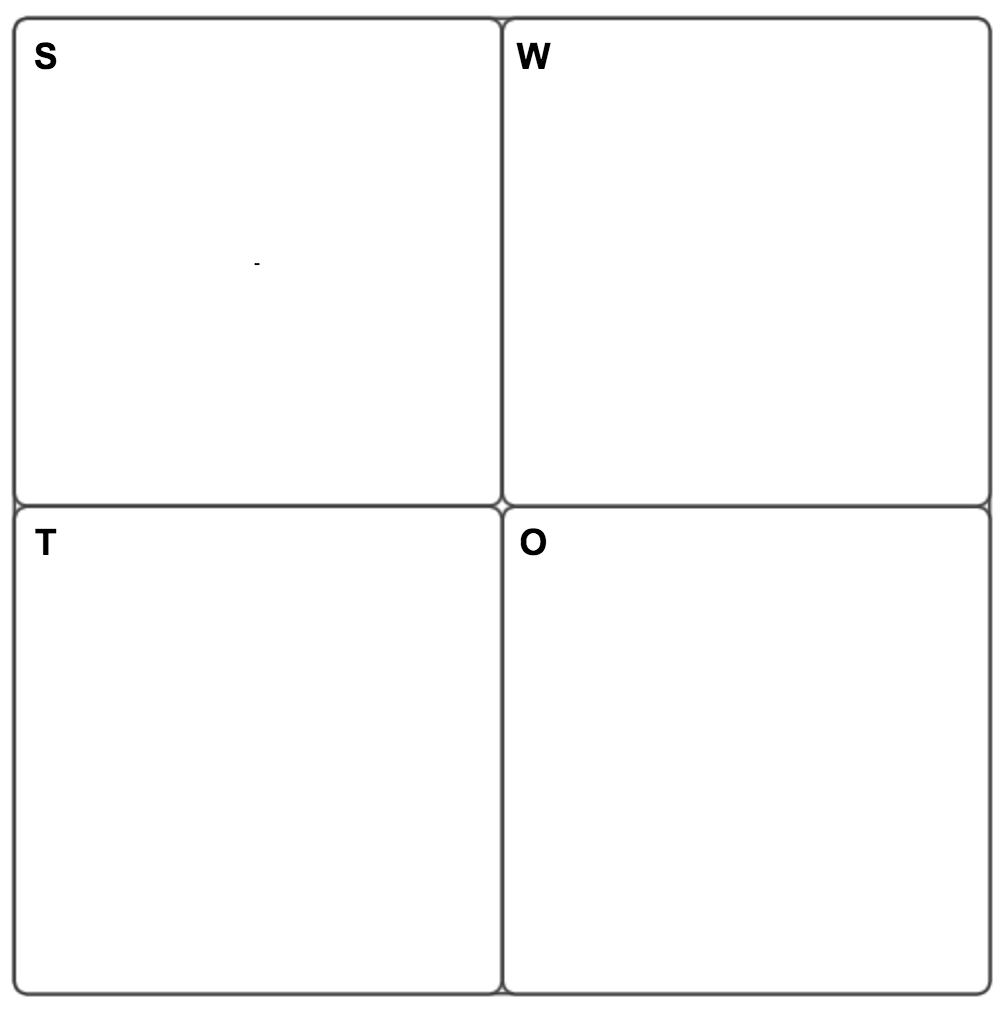
\includegraphics[scale=0.75]{img/generalswot}}
\label{fig:swotusuarios}
\caption* {Fonte: Elaborado pelo próprio autor}
\end{figure}